% !TeX spellcheck = pl_PL
% Options for packages loaded elsewhere
\PassOptionsToPackage{unicode}{hyperref}
\PassOptionsToPackage{hyphens}{url}
%
\documentclass[a4paper,11pt]{article}
\usepackage{times,fullpage,polski}
\usepackage{amssymb,amsmath}

 \usepackage[T1]{fontenc}
\usepackage[utf8]{inputenc}
\usepackage{textcomp} % provide euro and other symbols


%\usepackage{ifxetex,ifluatex}
%\ifnum 0\ifxetex 1\fi\ifluatex 1\fi=0 % if pdftex
%  \usepackage[T1]{fontenc}
%  \usepackage[utf8]{inputenc}
%  \usepackage{textcomp} % provide euro and other symbols
%\else % if luatex or xetex
%  \usepackage{unicode-math}
%  \defaultfontfeatures{Scale=MatchLowercase}
%  \defaultfontfeatures[\rmfamily]{Ligatures=TeX,Scale=1}
%\fi
%% Use upquote if available, for straight quotes in verbatim environments
%\IfFileExists{upquote.sty}{\usepackage{upquote}}{}
%\IfFileExists{microtype.sty}{% use microtype if available
%  \usepackage[]{microtype}
%  \UseMicrotypeSet[protrusion]{basicmath} % disable protrusion for tt fonts
%}{}
%\makeatletter
%\@ifundefined{KOMAClassName}{% if non-KOMA class
%  \IfFileExists{parskip.sty}{%
%    \usepackage{parskip}
%  }{% else
%    \setlength{\parindent}{0pt}
%    \setlength{\parskip}{6pt plus 2pt minus 1pt}}
%}{% if KOMA class
%  \KOMAoptions{parskip=half}}
%\makeatother
%\usepackage{xcolor}
%\IfFileExists{xurl.sty}{\usepackage{xurl}}{} % add URL line breaks if available
\IfFileExists{bookmark.sty}{\usepackage{bookmark}}{\usepackage{hyperref}}
\hypersetup{
  hidelinks}
\urlstyle{same} % disable monospaced font for URLs
\usepackage{graphicx}
%\makeatletter
%\def\maxwidth{\ifdim\Gin@nat@width>\linewidth\linewidth\else\Gin@nat@width\fi}
%\def\maxheight{\ifdim\Gin@nat@height>\textheight\textheight\else\Gin@nat@height\fi}
%\makeatother
%% Scale images if necessary, so that they will not overflow the page
%% margins by default, and it is still possible to overwrite the defaults
%% using explicit options in \includegraphics[width, height, ...]{}
%\setkeys{Gin}{width=\maxwidth,height=\maxheight,keepaspectratio}
%% Set default figure placement to htbp
%\makeatletter
%\def\fps@figure{htbp}
%\makeatother
%\setlength{\emergencystretch}{3em} % prevent overfull lines
%\providecommand{\tightlist}{%
%  \setlength{\itemsep}{0pt}\setlength{\parskip}{0pt}}
%\setcounter{secnumdepth}{-\maxdimen} % remove section numbering


\newcommand{\ang}[1]{(ang. \emph{#1})}


\begin{document}


\title{Kwantowe obliczenia wariacyjne\\ {\normalsize Podstawowe zasady konstrukcji}}

\author{Jarosław Miszczak}
\date{11/11/2022}

\maketitle

\begin{abstract}
Raport przedstawia podstawowe koncepcje związane z kwantowymi algorytmami wariacyjnymi. Omówione są m.in. konstrukcja funkcji kosztu, typy ansatzów oraz proces optymalizacji.
\end{abstract}


%-------------------------------------------------------------------------------
\hypertarget{wprowadzenie}{%
\section{Wprowadzenie}\label{wprowadzenie}}
%-------------------------------------------------------------------------------

 Komputery które mogłyby wykonywać algorytmy numeryczne typu algorytmu Shora wymagają dużej ilości pamięci kwantowej odpornej na błędy \ang{fault-tolerant quantum computing} i w chwili obecnej uważa się, iż budowa takich komputerów nie będzie możliwa w najbliższej przyszłości. Natomiast komputer które są dostępne obecnie i będą dostępne w ciągu najbliższych lat będą dawały dostęp do pamięci rzędu kilkuset kubitów, a dodatkowo obliczenia kwantowe realizowane na nich będą wymagały radzenia sobie z szumem kwantowym. W związku z tym konieczne jest opracowanie algorytmów kwantowych, które będą konstruowane z myślą o tego typu urządzeniach, a ich zasada działania będzie uwzględniała ich ograniczenia.
 
 Wariacyjne algorytmy kwantowe \ang{Variational Quantum Algorithms -- VQA} stanowią główny trend w rozwoju algorytmów dla takich małych, zaszumionych komputerów najbliższej przyszłości \ang{Noisy Intermediate-Scale Quantum - NISQ}. Algorytmy tego dostarczają sposobu budowania rozwiązań dla szerokeij klasy problemów. Mogą być zatem dostosowane do różnych zastosowań, przy czym podstawowa struktura wszystkich tak zbudowanych algorytmów jest bardzo podobna.

\newpage 

%-------------------------------------------------------------------------------
\hypertarget{zasada-dzialania}{%
	\section{Zasada działania}\label{zasada-dzialania}}
%-------------------------------------------------------------------------------

\begin{figure}[h!]
	\centering
	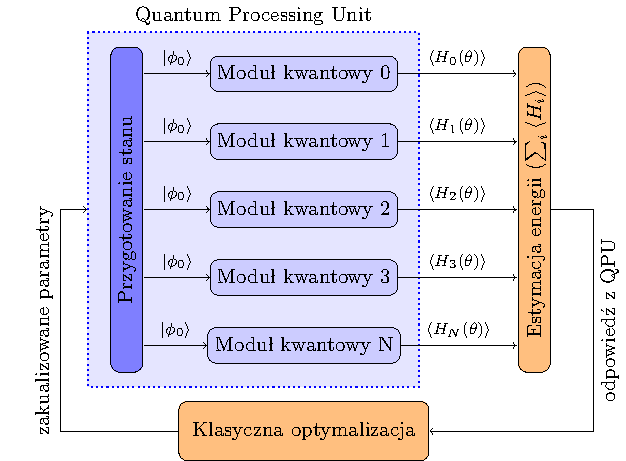
\includegraphics[width=0.5\textwidth]{vqe-pl.pdf}
	\caption{Koncepcja działania kwantowego algorytmu wariacyjnego}
\end{figure}

\newpage 

%-------------------------------------------------------------------------------
\hypertarget{funkcja-kosztu}{%
	\section{Funkcja kosztu}\label{funkcja-kosztu}}
%-------------------------------------------------------------------------------

Podstawowym elementem każdego kwantowego algorytmu wariacyjnego jest określenie funkcji kosztu. Podobnie jak w przypadku klasycznego treningu modelu, funkcja kosztu mapuje wartości parametrów $\mathbf{\theta}$ na zbiór liczb rzeczywistych. Funkcja kosztów jest skonstruowana tak, że znalezienie parametrów ansatzu, które minimalizują jej wartość, rozwiązuje interesujący nas problem.  W ogólności funkcja kosztu może być wyrażona w postaci
\begin{equation}
	C(\theta)  = f(\{\rho_k\}, \{O_k\}, U(\theta))
\end{equation}
gdzie $f$ to dowolna funkcja, $\rho_k$ to zestaw stanów wejściowych, a $O_k$ to obserwable.

Aby funkcja kosztu była dobra do wykorzystania w wariacyjnym algorytmie kwantowym, powinna spełniać następujące warunki:
\begin{itemize}
	\item wierność -- 
	\item wydajność estymacji -- 
	\item znaczenie operacyjne --
	\item trenowalność -- 
\end{itemize}


\paragraph{Wierność}
\paragraph{Wydajność estymacji}
\paragraph{Znaczenie operacyjne}
\paragraph{Trenowalność}

\newpage 

%-------------------------------------------------------------------------------
\hypertarget{typy-ansatzow}{%
	\section{Ansatz}\label{typy-ansatzow}}
%-------------------------------------------------------------------------------

Jednym z kluczowych elementów projektowanie algorytmu opartego na metodzie wariacyjnej jest dobranie odpowiedniego schematu obwodu, którego parametry będą poddawane procesowi optymalizacji. Schemat ten nazywany jest \emph{ansatzem}.


\begin{figure}[ht!]
	\centering
	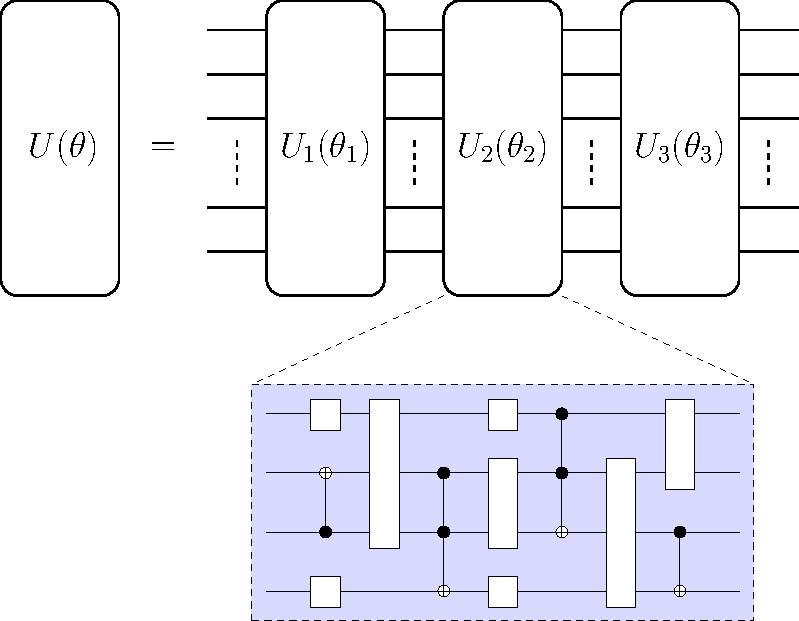
\includegraphics[width=0.5\textwidth]{ansatz.pdf}
	\caption{Zasada konstrukcji ansatzow w wariacyjnych algorytmach kwantowych}
\end{figure}


Struktura ansatza zależy od problemu który mamy zadanie rozwiązać. W związku z tym możemy wyróżnić ansatze inspirowane problemowo.



%-------------------------------------------------------------------------------
\subsection{Ansatz wydajny sprzętowo}
%-------------------------------------------------------------------------------

Ansatz wydajny sprzętowo \ang{hardware efficient ansatz -- HEA} to ogólna nazwa rodziny ansatzów w konstrukcji których wykorzystywana jest wiedza na temat architektury komputera kwantowego na którym będzie realizowany algorytm. Wiedza ta pozwala na zminimalizowanie głębokości obwodów dla danej architektury komputera kwantowego. Ponieważ zmniejszenie głębokości przekłada się na ograniczenie wpływu szumu kwantowego na jakość wykonywanych obliczeń, to podejście jest ważne jeżeli celem jest jak najwierniejsze wykonanie założonego zestawu operacji kwantowych.

W przypadku tego typu ansatzów pojawiają się często problemy ze zbieżnością, zwłaszcza przy losowej inicjalizacji parametrów.

%-------------------------------------------------------------------------------
\subsection{Warstwowy ansatz wydajny sprzętowo}
%-------------------------------------------------------------------------------

W przypadku warstwowego ansatz wydajnego sprzętowo \ang{layered hardware efficient ansatz -- LHEA} dodadkowo zakłada się, iż operacje wykonywane są naprzemiennie na kubitów. Prowadzi to do struktury przypominającej układ cegieł.  

%-------------------------------------------------------------------------------
\subsection{Kwantowy naprzemienny ansatz operatorowy}
%-------------------------------------------------------------------------------

Kwantowy naprzemienny ansatz operatorowy \ang{quantum alternating operator anzatz} bazuje na strukturze produktowej podyktowanej wykorzystaniem tzw. troteryzacji. Troteryzacja to metoda przybliżania wartości $e^{Ht}$ jako
\begin{equation}
	e^{Ht} \approx \left(e^{\frac{Ht}{n}}\right)^n.
\end{equation}


%-------------------------------------------------------------------------------
\subsection{Ansatz UCC}
%-------------------------------------------------------------------------------

%-------------------------------------------------------------------------------
\subsection{Wariacyjny anzatz hamiltonowski}
%-------------------------------------------------------------------------------

Wariacyjny anzatz hamiltonowski \ang{Hamiltonian Variational Ansatz -- HVA} jest inspirowany przez QAOA.


\newpage
%-------------------------------------------------------------------------------
\hypertarget{optymalizacja}{%
	\section{Optymalizacja}\label{optymalizacja}}
%-------------------------------------------------------------------------------


Problem optymalizacji jest kluczowy w trenowaniu wariacyjnych algorytmów kwantowych. Wykazano, że klasyczne problemy optymalizacyjne odpowiadające VQA i QAOA są NP-trudne. Co więcej, pokazano, że dla każdego algorytmu działającego w czasie wielomianowym istnieją instancje, dla których błąd względny wynikający z klasycznego problemu optymalizacyjnego może być dowolnie duży przy założeniu $\mathbf{P} \not= \mathbf{NP}$. Wskazuje to, że klasyczna optymalizacja w wariacyjnych algorytmach kwantowych jest fundamentalnie trudna, a nie tylko dziedziczy trudność po problemie znajdowania stanu podstawowego.


\newpage 



\hypertarget{literatura}{%
\section*{Literatura}\label{literatura}}

\begin{enumerate}
\def\labelenumi{\arabic{enumi}.}
%\tightlist

\item Cerezo, M., Arrasmith, A., Babbush, R., Benjamin, S.C., Endo, S., Fujii, K., McClean, J.R., Mitarai, K., Yuan, X., Cincio, L. and Coles, P.J., 2021. Variational quantum algorithms. Nature Reviews Physics, 3(9), pp.625-644. \url{https://doi.org/10.1038/s42254-021-00348-9}

\item Tilly, J., Chen, H., Cao, S., Picozzi, D., Setia, K., Li, Y., Grant, E., Wossnig, L., Rungger, I., Booth, G.H. and Tennyson, J., 2022. The variational quantum eigensolver: a review of methods and best practices. Physics Reports, 986, pp.1-128. \url{https://doi.org/10.1016/j.physrep.2022.08.003}

% VAE

\item Peruzzo, A., McClean, J., Shadbolt, P., Yung, M.H., Zhou, X.Q., Love, P.J., Aspuru-Guzik, A. and O’brien, J.L., 2014. A variational eigenvalue solver on a photonic quantum processor. Nature communications, 5(1), pp.1-7. \url{https://doi.org/10.1038/ncomms5213}


% HVA 
\item Wiersema, R., Zhou, C., de Sereville, Y., Carrasquilla, J.F., Kim, Y.B. and Yuen, H., 2020. Exploring entanglement and optimization within the hamiltonian variational ansatz. PRX Quantum, 1(2), p.020319. \url{https://doi.org/10.1103/PRXQuantum.1.020319}

\item Wecker, D., Hastings, M.B. and Troyer, M., 2015. Progress towards practical quantum variational algorithms. Physical Review A, 92(4), p.042303. \url{https://doi.org/10.1103/PhysRevA.92.042303}


% optimization

\item Bittel, L. and Kliesch, M., 2021. Training variational quantum algorithms is np-hard. Physical Review Letters, 127(12), p.120502. \url{https://doi.org/10.1103/PhysRevLett.127.120502}

% applicaitons


\end{enumerate}

\end{document}
